\documentclass[a4paper,12pt]{report}
\usepackage[utf8]{inputenc}
\usepackage[magyar]{babel}
\usepackage{t1enc}
\usepackage{graphicx}
\usepackage{amssymb}
\usepackage{url}
\usepackage{setspace}

\usepackage{color}
\usepackage{xcolor}
\usepackage{listings}
\usepackage{couriers}
\lstset{language=c++,
basicstyle=\footnotesize\ttfamily,
stepnumber=1,
firstnumber=0,
numbersep=5pt,
numbers=left,
showspaces=false,
showstringspaces=false,
showtabs=false,
tabsize=3,
breaklines=true,
breakatwhitespace=false,
float,
frame=linesc,
%keywordstyle=\color{blue}
keywordstyle=\bfseries
}

\definecolor{bground}{rgb}{0.92,0.92,0.92}

\newcommand{\pelda}[6]{%
\begin{figure}[ht!]
\centering
\framebox{%
\colorbox{bground}{%
\begin{minipage}{#1}%
\end{minipage}%
}%
}%
\label{#6}
\caption{#5}
\end{figure}
}

\newcommand{\lexelements}[2]{%
\null\smallskip
\framebox{%
\colorbox{bground}{%
\begin{minipage}{0.9\textwidth}%
\textbf{#1} \\%
\null\\%
\begin{footnotesize}
#2%
\end{footnotesize}
\end{minipage}%
}%
}%
}


\setlength{\textwidth}{140mm}
\setlength{\textheight}{237mm}
\usepackage[top=30mm, bottom=30mm, left=40mm, right=30mm]{geometry}
\usepackage{setspace}


\sloppy
\linespread{1.3}

% Title Page
\title{Dokumentáció}
\author{Bodor Zoltán, Hack János, Nagy Márton, Pető Bence}

\begin{document}
\maketitle

%\input{cimlap.tex}

\tableofcontents

\chapter{Követelmény Feltárás}

a fajok részletes leíását tartalamző txt tartalam valahova sztem ide kell de nem tudom pontossan hova ....

\section{Célkitűzés, projektindító dokumentum}

A szoftver egy egy számítógépnél játszható körökre osztott startégiai játék lesz. A megrendelő elvárja a játéktól, hogy több ember, legalább kettő, képes legyen egymás ellen játszani. A felhasználó
szeretne a játékban a saját választott nevével játszani. A játék egy pályán játszódik, ahol a játékosok különböző egységekkel rendelkeznek. A játék célja a másik játékos egységeinek legyőzése, vagy a pályán megtalálható pénzbeviteli források teljes uralma.
A megrendelő további az alap játékon túli feature-öket is szívessen látna az ídő és erőforrás mennyiségétől függően. Ezek a következőek lennének:
\begin{itemize}
\item Saját pályák készítésének lehetősége.
\item A megkezdett játékok elmentése, valamint visszatöltése.
\item Játékos ranglétra, amin a legjobb 10 játékos látszik elért pont alapján.
\item Csata közbeni súgó, amin meg tudja nézni agy egységek részletes leírását és a részletes játék szabályokat.
\item Játék gépi játékos ellen, valamint 2 vs 2, hogy több ismerősével is játszhasson.
\end{itemize} 

\section{Szakterületi fogalomjegyzék}

\begin{itemize}
\item {\bf Hotseat}: Egy számítógép előtti, egy billenytűzettel és egérrel játszható, többjátékos mód.
\item {\bf Race}: A játékban használható fajok.
\item {\bf Lader}: A játékos ranglétra, itt szerepelnek a legjobb játékosok.
\item {\bf Körökre osztott stratégia}: A játék körökből áll, egy kör egy játékos összes lépését jelenti a tovább adásig a másik játékosnak.
\end{itemize}

\section{Használatieset-modell, funkcionális követelmények}

A Szoftver alapvető célja a játék. A Játék alapértelmezett eseben egy számítógép előtt ülő két emberek között zajlik. A játékosok választhatnak maguknak nevet a játék megkezdése előtt,
ha nem választanának a játék az alapértelmezett neveket használja majd (Player1, Player2), amivel később a játékban hivatkozunk rájuk. A játékosok a nevük megválasztása után választhatnak az előre elkészített pályák közül, valamint random is generáltathatnak pályát, amin játszani fognak. A pálya kiválasztása után minden játékosnak
lehetősége nyilik a játszani kívánt faj kiválasztására. Ezután megkezdődhet a játék.

A felhasználó továbbá extra featureként szívessen látná a következő dolgokat:
\begin{itemize}
\item Saját pályák készítésének lehetősége.
\item A megkezdett játékok elmentése, valamint visszatöltése.
\item Játékos ranglétra, amin a legjobb 10 játékos látszik elért pont alapján.
\item Csata közbeni súgó, amin meg tudja nézni agy egységek részletes leírását és a részletes játék szabályokat.
\item Játék gépi játékos ellen, valamint 2 vs 2, hogy több ismerősével is játszhasson.
\end{itemize} 

\begin{figure}[hbtp]
\centering
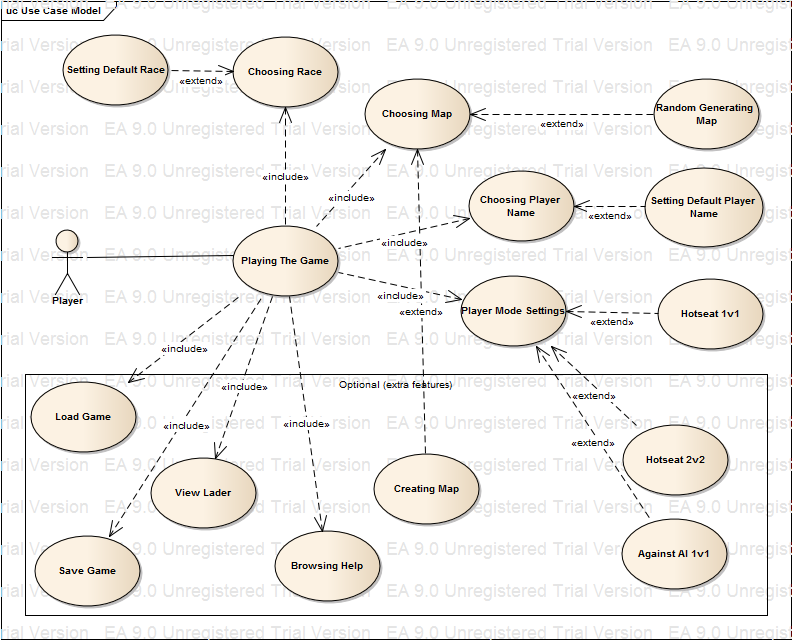
\includegraphics[width=1\textwidth]{UseCaseModel.png}
\caption{Használatieset-modell}
\label{fig:hmm}
\end{figure}

\begin{figure}[hbtp]
\centering
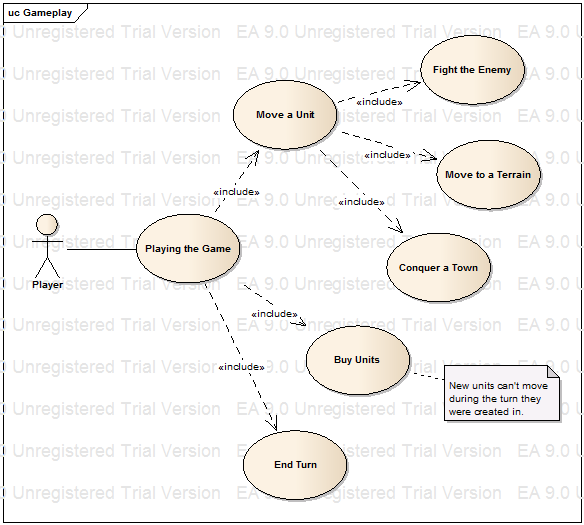
\includegraphics[width=1\textwidth]{GamePlayUseCase.png}
\caption{Játékmenet használatieset-modell}
\label{fig:hmm}
\end{figure}

\section{Szakterületi követelmények}

\section{Nem funkcionális követelmények}
\begin{itemize}
\item A játék legyen könnyen átlátható, és használata a gyorsan tanulható.
\end{itemize} 

\chapter{Tervezés}

\section{Program architecturája}

A program három fő komponensből tevődik össze melyek az MVVM (Model-View-ViewModel) minta alap elemei. A kapcsolatok az egyes komponensek között a tervmintának megfelelően a következőek:
\begin{itemize}
\item {\bf Model}: Az üzleti logika – a játék eseményeinek kezelése, számítások stb. – ebben a komponesben található. Ide kerül minden a játék logikai működéséért felelős osztály.
\item {\bf View}: Minden a megjelenítéssel kapcsolatos osztály, a különböző megjelenítendő sémák osztályai.
\item {\bf ViewModel}: A View és Model komponest köti össze, az ide tartozó osztályok felelősek a két téteg együttműködésért, semilyen számítást végző osztályt vagy felületi elemet nem tartalmazhat.
\end{itemize}
 
\section{Osztálymodell}

\subsection{View}

\begin{figure}[hbtp]
\centering
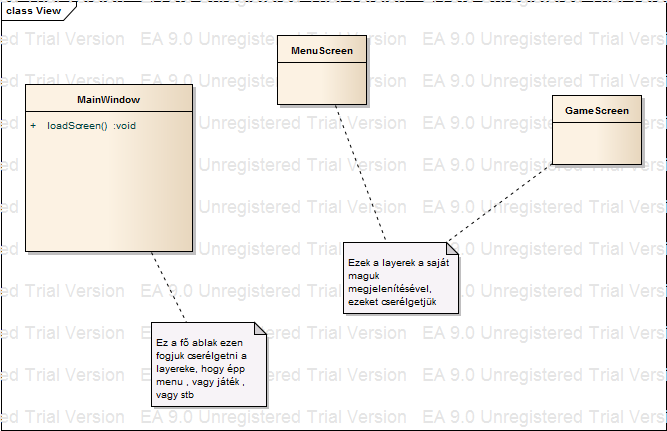
\includegraphics[width=1\textwidth]{ViewClass.png}
\caption{View Osztálydiagram}
\label{fig:vc}
\end{figure}

\subsection{Model}

A Model névtér tartalmazza a játék logikájához szükséges osztályokat. Itt tároljuk az aktuális játékállást, a térképet, a játékosok egységeit stb.

Gyakorlatilag egy kiszolgáló, egyetlen példány létezik belőle (singleton), minden adatbáziskérés vagy háttéradat-módosítás itt történik. Van néhány funkció, ami visszaad értéket a ViewModelnek, a többi csak frissíti az adatagokat amik hozzá vannak kötve a ViewModelen kereszül a Viewhoz, és ha frissülnek szól a Viewnak, ami mindent lefrissít a változtatásoknak megfelelően.

\begin{figure}[hbtp]
\centering
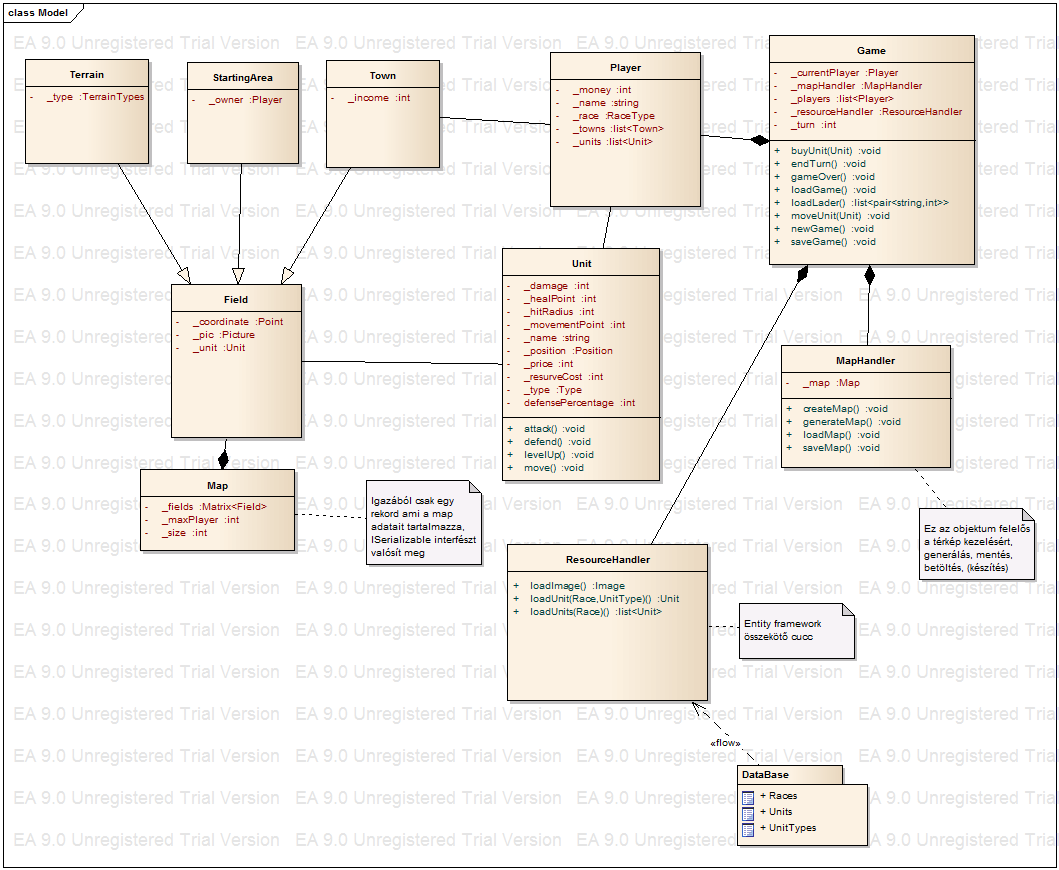
\includegraphics[width=1\textwidth]{ModelClass.png}
\caption{Model Osztálydiagram}
\label{fig:mc}
\end{figure}

\subsubsection{Unit}
A Unit osztály írja le az egységeket. Az egység három különböző faj lehet, mindegyik három szintű lehet. A Unit osztályból mindig az összes létező egység számával megegyező példány létezik. Feladata egy adott egység tulajdonságainak tárolása.

\begin{figure}[hbtp]
\centering
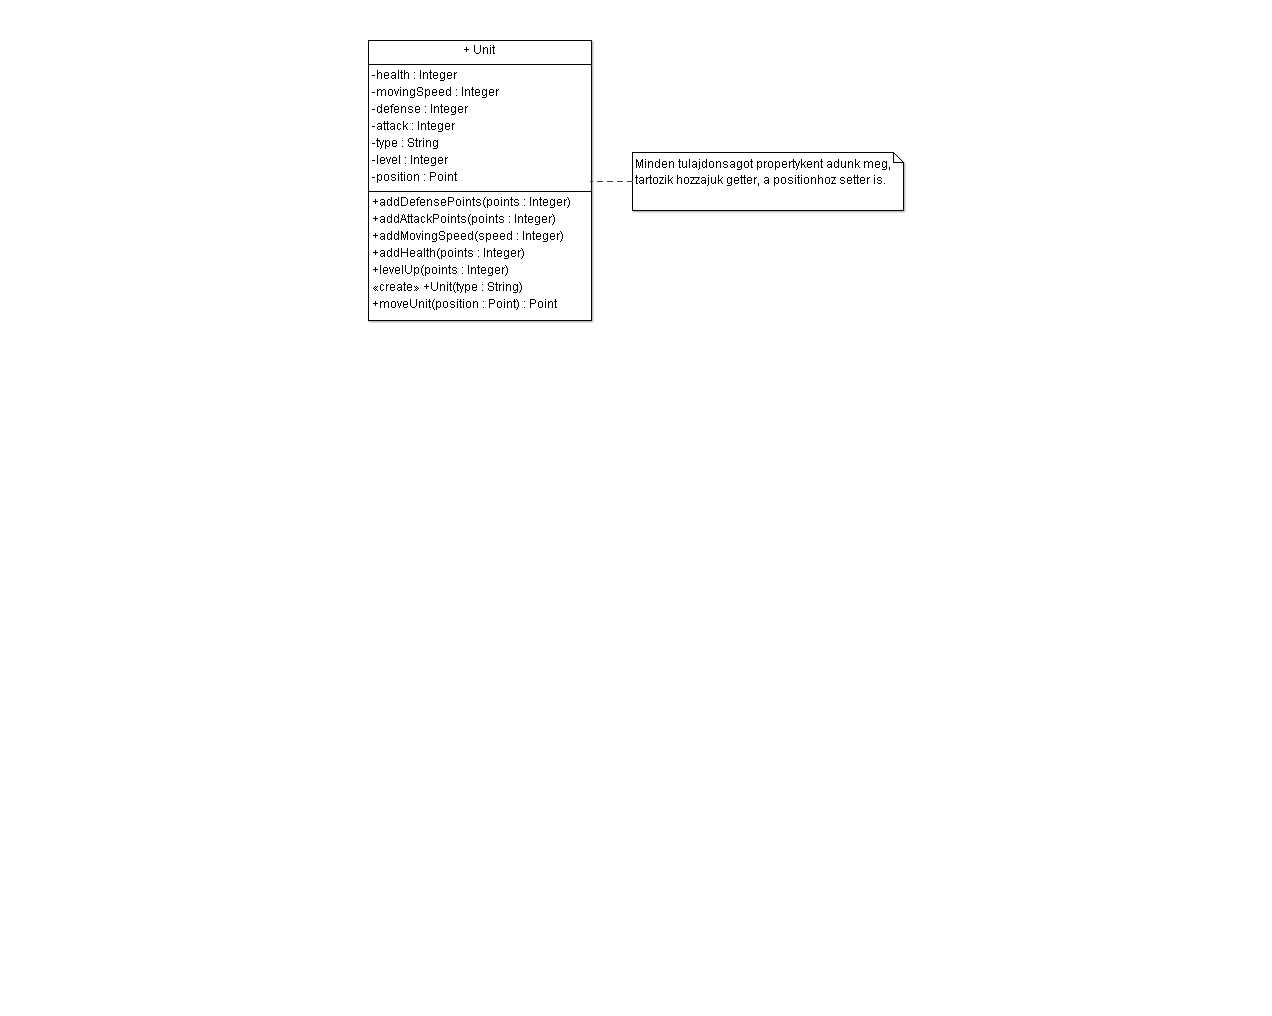
\includegraphics[width=1\textwidth]{Unit.png}
\caption{Unit osztály}
\label{fig:unitclass}
\end{figure}

A tulajdonságokat property-kben tároljuk, amiket getterrel és setterrel érünk el.

A fajokat egy felsoroló típus írja le. A faj három féle lehet: ELF/HUMAN/ORC.

Minden fajon belül négy típusú egységet hozhatunk létre. Ennek tárolására is egy felsorolási típust használunk, melynek elemei: ATTACKER/DEFENDER/SUPPORTER/SCOUT.

A konstruktor a fenti két paraméter segítségével hozza létre az egységeket a megfelelő tulajdonságokkal.

A MoveUnit metódus felelős az egység elmozdításáért. Paraméterül az új helyet és a mozgás költségét kapja. Ha a mozgás költsége nagyobb, mint a rendelkezésre álló mozgáspont, az egység helyben marad, egyébként elmozdul a megadott helyre. Visszatérési értéke igaz, ha a mozgás sikerült, egyébként hamis.

A HealUnit metódus "gyógyítja" az egységeket. Paraméterül egy egész számot kap, ennyivel kell növelni az egység életerejét.

A LevelUp függvény felelős az egységek szintlépéséért. Meghívásakor az egység megfelelő tulajdonságai megnöveli.

\subsubsection{Game}
A Game osztályhoz fut be minden kérés, ő a Model lelke, ellenőrzi a kívánt műveletek (lépések stb.) érvényességét, frissíti a térképen lévő egységeket, mezőket, magát a térképet, amely változtatásokról a View értesül.

Képes a játék állásának minden összetevőjét közvetlenül vagy közvetetten elérni, bizonyos dolgokat önmaga is tárol a játékállásról.

Adattagjai:
\begin{itemize}
\item \textit{currentPlayer}: A játékban soron lévő játékos. A jelenlegi játékállásban a következő lépés csak számára engedélyezett; ha más próbál lépni, az nem megengedett művelet.
\item \textit{mapHandler}: A Game ezen az osztályon keresztül lép kapcsolatba a térképpel, hiszen ő felelős a térkép kezeléséért: generálás, mentés, betöltés.
\item \textit{players}: A játékosok listája. A Game őket arra használja, hogy pl. az adott lépést képes-e a játékos a meglévő pénzével, fajával stb. megtenni. A Game rajta keresztül látja a Unitokat is.
\item \textit{resourceHandler}: A Game ezt az osztályt használja a bináris adatok, és az adatbázisban tárolt adatok betöltésére.
\item \textit{turn}: A jelenlegi kör száma.
\end{itemize}

Metódusai:
\begin{itemize}
\item \textit{newGame()}: A játék elején hívódik meg, durván egy logikai konstruktornak is tekinthető. Létrehozza a játék elején szükséges objektumokat, beállítja a játékosok, egységek stb. alapértelmezett értékeit.
\item \textit{loadGame()}: Betölt egy korábban elmentett játékállást. Létrehozza a szükséges objektumokat, beállítja az értéküket, a MapHandler-rel legeneráltatja a térképet stb.
\item \textit{saveGame()}: Menti a jelenlegi játékállást úgy, hogy később betölthető legyen, ld. loadGame().
\item \textit{gameOver()}: A játék végén hívódik meg, durván egy logikai destruktornak is tekinthető. Elvégzi a játék végén fontos teendőket; pl. frissíti a Lader-t, felszabadítja az erőforrásokat stb.
\item \textit{endTurn()}: Minden kör végén hívódik meg. A teljesítmény alapján a játékosok pénzt kapnak, illetve az egységeik száma alapján zsoldot fizetnek.
\item \textit{moveUnit()}: Az egységek mozgatásához használt metódus. A mozgással lehet falvat foglalni, az ellenséggel harcolni, vagy egyszerűen másik mezőre lépni. Ezek mindegyike másféleképp befolyásolja az egységek tulajdonságait.
\item \textit{buyUnit()}: Egységek vásárlásakor hívott metódus. Létrehozza az új egységet, és lehelyezi a térkép speciális részére, a játékos kezdőterületére.
\end{itemize}

\subsection{ViewModel}

\begin{figure}[hbtp]
\centering
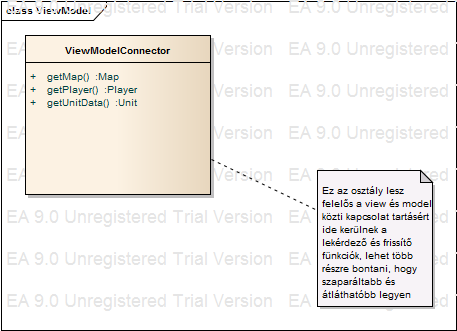
\includegraphics[width=1\textwidth]{ViewModelClass.png}
\caption{ViewModel Osztálydiagram}
\label{fig:vmc}
\end{figure}

\section{Dinamkus működés}

\section{Felhasználó-felület modell}

\begin{figure}[hbtp]
\centering
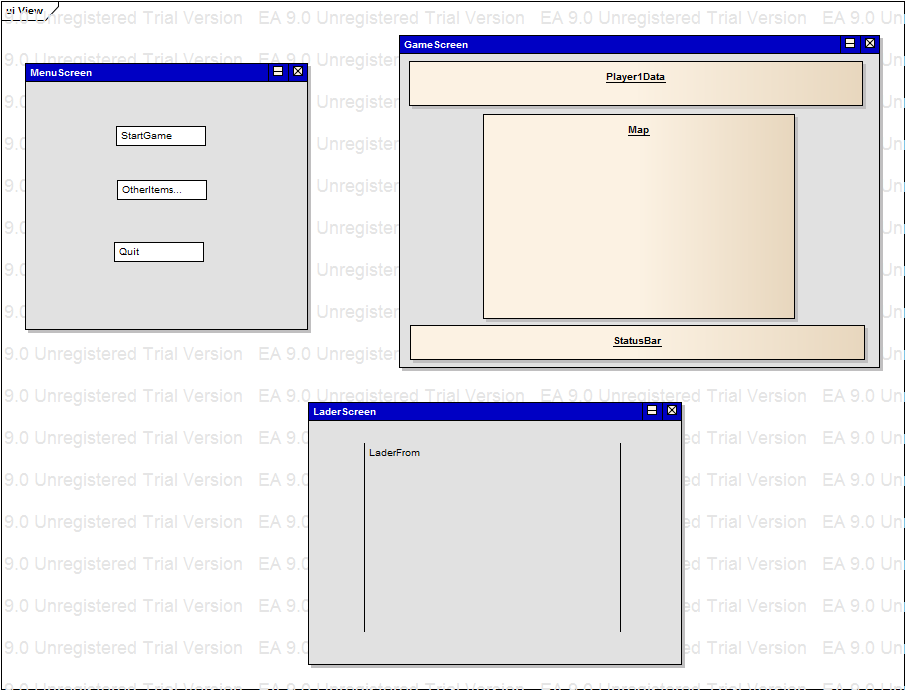
\includegraphics[width=1\textwidth]{ViewScreen.png}
\caption{Felület Tervek}
\label{fig:vs}
\end{figure}

\section{Részletes programterv}


\end{document} 
